
%%%%%%%%%%%%%%%%%%%%%%% file typeinst.tex %%%%%%%%%%%%%%%%%%%%%%%%%
%
% This is the LaTeX source for the instructions to authors using
% the LaTeX document class 'llncs.cls' for contributions to
% the Lecture Notes in Computer Sciences series.
% http://www.springer.com/lncs       Springer Heidelberg 2006/05/04
%
% It may be used as a template for your own input - copy it
% to a new file with a new name and use it as the basis
% for your article.
%
% NB: the document class 'llncs' has its own and detailed documentation, see
% ftp://ftp.springer.de/data/pubftp/pub/tex/latex/llncs/latex2e/llncsdoc.pdf
%
%%%%%%%%%%%%%%%%%%%%%%%%%%%%%%%%%%%%%%%%%%%%%%%%%%%%%%%%%%%%%%%%%%%


\documentclass[runningheads,a4paper]{llncs}

\usepackage{amssymb}
\setcounter{tocdepth}{3}
\usepackage{graphicx}

\usepackage{url}
\urldef{\mailsa}\path|{rainer.poisel,simon.tjoa}@fhstp.ac.at|
\newcommand{\keywords}[1]{\par\addvspace\baselineskip
\noindent\keywordname\enspace\ignorespaces#1}

\begin{document}

\mainmatter  % start of an individual contribution

% first the title is needed
\title{Discussion on the Challenges and Opportunities of Cloud Forensics}

% a short form should be given in case it is too long for the running head
\titlerunning{Lecture Notes in Computer Science: Authors' Instructions}

% the name(s) of the author(s) follow(s) next
%
% NB: Chinese authors should write their first names(s) in front of
% their surnames. This ensures that the names appear correctly in
% the running heads and the author index.
%
\author{Rainer Poisel (rpoisel)\and Simon Tjoa (stjoa)}
\institute{Institute of IT Security Research\\
St. Poelten University of Applied Sciences\\
St. Poelten, Austria\\
\mailsa\\
\url{http://www.fhstp.ac.at}}
%
\authorrunning{Discussion on the Challenges and Opportunities of Cloud Forensics}
% (feature abused for this document to repeat the title also on left hand pages)

% the affiliations are given next; don't give your e-mail address
% unless you accept that it will be published

%
% NB: a more complex sample for affiliations and the mapping to the
% corresponding authors can be found in the file "llncs.dem"
% (search for the string "\mainmatter" where a contribution starts).
% "llncs.dem" accompanies the document class "llncs.cls".
%

\toctitle{Discussion on the Challenges and Opportunities of Cloud Forensics}
\tocauthor{Cloud Forensics}
\maketitle


\begin{abstract}
Cloud Forensics refers to digital forensics investigations performed in Cloud Computing Environments. Nowadays digital investigators face various technical, legal, and organizational challenges to keep up with current developments in the field of Cloud Computing. But, due to its dynamic nature, Cloud Computing also offers several opportunities to improve digital investigations in Cloud Environments. Digital investigators may utilize Cloud Computing setups and process complex tasks in cloud infrastructures. Thus they can take advantage of the enormous computing power at hand in such environments. 

In this paper we focus on the current State-of-the-Art of affected fields of Cloud Forensics. The benefit for the reader of this paper is a clear overview of the challenges and opportunities for scientific developments in the field of Cloud Forensics. 
\keywords{Cloud Forensics, digital forensics, evidence}
\end{abstract}

\section{Introduction}

In recent years, Cloud Computing has gained vastly in importance. It has been introduced to optimize the general usage of IT infrastructures. Cloud Computing is a technology that evolved from technologies of the field of distributed computing, especially grid computing \cite{Foster2009}. According to NIST \cite{Mell2011}, ``Cloud Computing is a model for enabling ubiquitous, convenient, on-demand network access to a shared pool of configurable computing resources (e. g. networks, servers, storage, applications, and services) that can be rapidly provisioned and released with minimal management effort or service provider interaction''

There will be substantial market growth in the field of Cloud Computing over the next few years. According to Kazarian and Hanlon \cite{Kazarian2010}, 40\% of small and medium businesses (SMBs) from different countries are expected to use three or more cloud services and migrate their data into the cloud. In 2010, Gartner \cite{Gartner2010} released a study which forecasted the cloud service revenues to reach 148.8 billion in 2014 (compared to 58.6 billion in 2009). Carlton and Zhou \cite{Carlton2011} state that Cloud Computing is, from a technical point of view, a combination of existing technologies. People have difficulties to capture the big picture: for managers and customers of cloud services the idea is similar to exchanging information through web-based user interfaces. Others view the concept as being an extension of the timesharing concept from the 1960s. 

Cloud providers sell services based on different business models (also referred to as ``service models''): Software-as-a-Service (SaaS), Platform-as-a-Service (PaaS), and Infrastructure-as-a-Service (IaaS) \cite{Mason2011,Dillon2010}. With SaaS, the customer uses applications which are provided by the service seller (e. g. web-based e-mail services). With PaaS, the service seller then provides his infrastructure (servers, operating systems, network, etc.). The customer is able to write/use his own applications using the application programming interface made available by the provider. IaaS enables the user to use and run software of his choice (e. g. operating systems). The service seller provides the customer with the necessary infrastructure (servers, network, storage facilities, etc). 

Depending on the level of access to the underlying cloud infrastructure the following types of clouds have been categorized \cite{Mason2011,Krutz2010}: private clouds, community clouds, public clouds, and hybrid clouds. In ``private clouds'' the infrastructure is operated on behalf of a single entity. Usually the infrastructure is located in the premises of the organization. ``Community clouds'' refer to cloud deployments where the infrastructure is shared by several organizations. In ``Public Clouds'' one or more providers run the infrastructure and make it available to anybody who wishes to pay for the service. ``Hybrid clouds'' refer to setups which are formed out of two or more cloud infrastructures. These in turn can be private, community, or public clouds. Of course, the shift in intercommunications and interaction between IT systems poses new challenges for digital forensics investigations. Cloud Service Providers (CSPs) often do not let their customers look behind their ``virtual curtains'' \cite{Birk2011}. Vendor dependent implementations, multiple jurisdictions and proprietary data exchange formats \cite{Beebe2009} bring digital forensics into a deeper crisis as it is already facing \cite{Garfinkel2010}. Ruan et al. \cite{Ruan2011} defined Cloud Forensics as being a cross discipline between Cloud Computing and digital forensics. It is further recognized as a subset of network forensics \cite{Lillard2010}. Network forensics deals with investigating private or public networks and as Cloud Computing is based on broad network access it should follow the main phases of the network forensic process. Delport et al. \cite{Delport2011} deem Cloud Forensics to be a subset of computer forensics as clouds consist of several nodes which are computers. This means that Cloud Forensics combines both, computer forensics and network forensics \cite{BBC2000}. 

Ruan et al. \cite{Ruan2011} further extended the definition of Cloud Forensics across three major dimensions: technical, legal, and organizational. The technical dimension describes the set of procedures and tools which are utilized to carry out the digital forensics process in cloud environments. The organizational dimension refers to the fact that Cloud Computing involves at least two parties: CSPs and cloud customers. Further it is possible that CSPs outsource some of their services to other CSPs. The legal dimension refers to multi-jurisdiction and multi-tenancy challenges. Both fields have been exacerbated in cloud environments. Existing agreements and regulations have to be adopted for forensics activities to not breach any jurisdictions or confidentiality measures.

This paper is structured into two parts. First we focus on the current State-of-the-Art of affected fields of Cloud Forensics. In the second part, based on the current State-of-the-Art, related challenges and opportunities are identified in order to derive and describe open research problems. 

\section{State of the Art of Cloud Forensics}

\label{sota}

This chapter describes the State-of-the-Art of affected fields of digital forensics investigations in cloud environments. 

\subsection{Existing Digital Forensics Frameworks}

Digital investigations have to consider various perspectives (e.g. legal perspective, technological perspective) in order to be successful. In order to coordinate the efforts between the various stakeholders, there exist a variety of publications dealing with procedures how to handle, analyze, document and present digital evidence. The presented work in this subsection contains well-known and well-established guidelines which are not specifically tailored to Cloud Computing. To some extent the principles introduced are also valid for cloud technology. However, an adaption of the organizational frameworks has to be considered to deal with the new challenges arising from the usage of Cloud Computing.

In the First Responder's Guide for Electronic Crime Scene Investigations \cite{NIST2001}, the forensic process is split into the four phases, (1) collection, (2) examination, (3) analysis and (4) report. The first phase is dedicated to capture electronic evidence. Thereafter, in the examination phase content and state of evidence is documented and the evidence is examined concerning hidden and obscured information. The last step of the second step is to reduce the information. In the analysis phase the evidence is analyzed concerning the relevance to the case. While examination is a technical task, analysis is usually conducted by an investigation team. Finally, in the last step reporting takes place \cite{NIST2001}. 

NIST SP800-86 \cite{Karen2006} shows how digital forensics can support incident handling. This publication focuses tackles digital forensics mainly from an IT perspective, not a legal perspective. The forensics process uses the phases of \cite{Karen2006}. 

Further widely-used digital forensic frameworks include the digital forensics framework of the Association of Chief Police Officers (ACPO) \cite{acpo-guidelines} and the DFRWS (Digital Forensics Research Workshop) Investigative Process model \cite{Carrier2003}. Cohen proposes, in \cite{Cohen2010}, a model consisting of the seven phases: identification, collection, transportation, storage, examination and traces, presentation, and destruction. Ke \cite{Ke2011} describes the application of the SABSA model to the digital forensics process to obtain forensically sound evidence. More information on digital forensics frameworks can be found in \cite{Pollitt2007}. 

\subsection{Investigation of Cloud Infrastructures}

According to Zimmerman and Glavach \cite{Zimmerman2011}, the technology of Cloud Computing is not new. It is a new way of providing applications and computing resources on demand. Therefore the technology seems a perfect solution for smaller businesses that do not have the necessary resources to completely fulfil their IT needs \cite{Biggs2009,Pollitt2008}. Further, it allows private end users to utilize massive amounts of computing resources at affordable prices. However, the introduction of new technologies poses new challenges for the digital forensics investigator \cite{Wolthusen2009}. Grispos et al. show ``how established digital forensic procedures will be invalidated in this new environment'' \cite{Grispos2011}. They propose research agendas for addressing the new challenges depending on the investigation phase. As mentioned in the previous section there exist several organizational digital investigations frameworks. In the following the different investigation steps: identification, preservation, examination, and presentation are elucidated regarding their implementation for the investigation of cloud environments. 

Identification, Preservation, and Acquisition: Grispos et al. outline in \cite{Grispos2011} the lack of frameworks to determine which elements were affected by IT specific crimes. The usage of conventional intrusion detection systems in the context of Cloud Computing infrastructures has been proposed by several authors \cite{Grispos2011}. The preservation and acquisition step deals with evidence collection from computer based systems. The increasing storage capacity of devices and computer systems are everlasting challenges in digital forensics investigations \cite{Grispos2011}. With the introduction of Cloud Computing systems this challenge is still ubiquitous: the elastic ability of Cloud Computing infrastructures allows the user to request additional data storage in a limitless fashion. 

The chain of custody documents how evidence was handled in the context of the digital investigations process \cite{Casey2011}. The documentation describes how evidence was collected, analyzed, and preserved to be approved in court. Due to the remote nature of Cloud Computing scenarios, assumptions that have been made with the investigation of traditional computer systems are not valid anymore \cite{Reilly2010}. Investigators usually had physical access to traditional computer systems \cite{Zimmerman2011}. Therefore they were able perform a live analysis or to remove storage devices for analyzing them in a forensics laboratory. Storage devices are accessed through a computer network. Digital investigators have to obtain control of cloud services before investigating them \cite{Ruan2011}. Depending on time an investigator requires to gain control of such a service, relevant evidence can be destroyed (deliberately or accidentially) by both, the service user and the cloud provider \cite{Grispos2011}. In this regard, IaaS deployments provide much more useful information for digital forensics investigations than PaaS or SaaS setups \cite{Birk2011,Birk2011a}. With PaaS or SaaS deployment scenarios, customers do not have any control of the underlying operating infrastructure. The amount of information from servers is limited and therefore, the client has to contribute to the investigation process. Besides the technical challenges, the lack of regulatory and legal frameworks complicate meeting the chain of custody requirements \cite{Wang2010}. 

In Forensics, 'live' acquisitions and investigations allow to obtain data stored in non-persistent memory such as process information or active network connections \cite{Barrett2010} as well as temporary data, such as file locks or web browsing caches \cite{Birk2011,Grispos2011}, RFC3227 \cite{Brezinski2002} explains several best practices regarding live investigation of systems in case of security incidents. 

However, traditional forensics guidelines require storage images to be forensically sound. Therefore bit-by-bit copies including a check sum are made from digital storage devices from instances in ``dead'' state (the system has been shutdown) to proof the unadulteratedness of digital evidence \cite{acpo-guidelines}. Traditional search and seizure procedures may be impractical for performing digital investigations in Cloud Computing environments. Digital evidence is stored in cloud data centres, desktop computers or mobile phones which could be out of physical control by the digital investigator \cite{Taylor2011}. As it is almost impossible to make a bit-by-bit copy of storage devices \cite{Zimmerman2011} the ACPO guidelines are rendered pointless when it comes to complete authenticity of digital evidence in cloud environments. Acquiring all storage devices from such a setup would be too time consuming for investigators and too disruptive for CSPs \cite{Grispos2011}. Usually cloud users are only offered remote access to the logical representation of their data. In most cases, the underlying physical infrastructure is transparent for the user. In the future, new methods will be needed to allow partial recovery of data from physical devices in accordance with accepted forensic principles. Therefore, forensics tools have to be hybrid of the current live and post-mortem analysis methods \cite{Zimmerman2011}. There will be a need for intelligent tools that note and predict artefacts based on heuristics. Delport et al. outline in \cite{Delport2011} that it might be necessary to isolate cloud instances in case they have to be investigated. The problem associated with isolating cloud instances is the integrity of data intended for digital forensics investigations \cite{Biggs2009}. 

Basically, methods for clearing include moving uninvolved instances or suspicious instances to other nodes. This way the CIA of other instances is protected, but it might result in loss of possible evidence. However, by moving instances, evidence is protected from being tampered by these moved instances. Delport et al. \cite{Delport2011} presented different techniques to isolate instances of cloud environments. 

Instance relocation means moving an instance inside a cloud environment by moving the data logically or by creating new and destroying old instances. Server farming refers to putting up a spare instance which offers the same functionality as the instance intended for digital investigations. By Sandboxing programs can run in an environment which they cannot escape. Man in the Middle (MitM) refers to placing an entity between a sender and a receiver. In the field of digital forensics this entity is placed between the cloud instance and the hardware of the cloud. Delport et al. \cite{Delport2011} conclude that none of their presented approaches fulfils every requirement for the investigation of cloud environments. However, depending on the case techniques may be combined to gain explicit access to a cloud instance. 

The usage of cryptography in cloud environments poses additional challenges. CSPs offer encryption as a security feature to their customers. All data is encrypted on the client's side. The key to the encrypted data is never stored in the cloud environment \cite{Agudo2011}. 

Deleted data represents another major challenge due to the volatility and elasticity of cloud environments. On one hand, data that has remotely been requested to be deleted can be a rich source of evidence as it can still be physically existing \cite{Grispos2011}. On the other hand it depends on the CSP how to proceed in the event of a user requesting his data to be deleted \cite{Birk2011,Zimmerman2011} (e. g. Google's policy includes the deletion of such data from both, its active and replication servers as well as of all pointers to this data). 

Reilly et al. \cite{Reilly2010} also mentioned the lack of tool support for dealing with digital investigations with cloud data centres. Currently, most tools are intended for examining data from traditional computer setups such as office or home computers. Taylor et al. \cite{Taylor2011} recommended to update existing tool suites such as EnCase or FTK to account for new developments in the field of Cloud Computing. 

Examination and Analysis: Forensic tool suites such as The SleuthKit, FTK or EnCase perform ``pattern matching'' and ``filtering'' of data that is existing in different types of memory. Evidence in cloud is manifold and will likely be similar to evidence found in traditional computer setups \cite{Grispos2011}: office application documents, file fragments, digital images, emails, and log file entries \cite{Marty2011}. Checksums are used to verify the integrity of objects (disk images, files, log entries, etc.) in the Cloud. Detecting file signatures of files in question or files which should be excluded from a digital forensics investigation are crucial for the filtering process. Hegarty et al. \cite{Hegarty2011} describe a method for adapting existing signature detection techniques for their usage in cloud environments. To detect files with a specific hash value a so called ``initialiser'' submits the target buckets (storage units of a cloud customer) as well as the hash value to a so called ``Forensic Cluster Controller'' which in turn distributes the job of finding files with that has value to so called ``Analysis Nodes''.

In the future investigating cloud infrastructures may be a task performed by cloud deployments. However, cloud customers may access applications offered in the Cloud from a myriad of different computer setups (mobile phones of different make, desktop PCs with different operating systems, etc.) \cite{Taylor2011}. 

Presentation: Digital evidence can be utilized in several ways: it can be submitted to court in the form of a report \cite{Carrier2003} or it may be used by an organization to improve corporate policies and support future investigations \cite{Wang2005}. Grispos et al. \cite{Grispos2011} highlight the need for a standard evaluation method for Cloud Forensics so that Cloud Forensics investigation results pass the Daubert principles \cite{Marsico2005}. Another challenge arises from explaining the Cloud Computing concept to a jury in court \cite{Reilly2010}. It may be difficult for a jury member to comprehend the concept as jury members will usually only have basic knowledge of how to use home PCs. 

\subsection{Digital Investigations using Cloud Infrastructures}

According to cloud security alliance \cite{CSA2011}, industry is heading forward to create Security-as-a-Service (SecaaS). The authors identified the following ten domains that are likely to interest consumer in the future: (1) Identity and Access Management Services; (2) Data Loss Prevention; (3) Web Security; (4) Email Security; (5) Security Assessments; (6) Intrusion Management, Detection and Prevention (IDS/IPS); (7) Security Information and Event Management; (8) Encryption; (9) Business Continuity and Disaster Recovery; (10) Network Security. Within one of these domains the authors identify the requirement to ``\ldots provide customers with forensics support\ldots''. This opinion is also supported by Ruan et al. \cite{Ruan2011} who derive from the emerging trend to security-as-a-service that forensics-as-a-service will gain importance in cyber criminal investigations by providing massive computing power.

Reilly et al. \cite{Reilly2010} take the discussion of the usage of cloud technologies for forensic investigations one step further and highlight the benefits delivered by the usage of Cloud Computing for digital investigations. The major advantages identified by the authors include large-scale storage, high availability and massive computing power. Roussev and Richard \cite{Roussev2004,Richard2006} recognized the need for distributed forensics at an early stage. In their paper \cite{Roussev2009} they formulated the following requirements that should be satisfied by a distributed digital forensic toolkit: Scalability, platform-independence, lightweight, interactivity, extensibility and robustness. As cloud technologies can meet the abovementioned requirements, Roussev et al. evaluate in their paper \cite{Roussev2009} the feasibility and applicability of MapReduce for forensics applications. Map Reduce \cite{Dean2004} was developed by Google in order to facilitate large scale computing. Phoenix \cite{Talbot} and Hadoop \cite{Hadoop2011a} are well known implementations of Google's MapReduce model. In their paper, the authors present their prototype, called MPI MapReduce (MMR), which is based on the Phoenix shared memory implementation. In order to test the performance of the prototype they implemented three Hadoop samples (wordcount, pi-estimator and grep) for MMR. 

Cohen et al. introduce in \cite{Cohen2011} their GRR Rapid Response framework which pursues the objective to support live forensics within in an enterprise. The framework is designed to be highly scalable and is available for all common platforms. The proposed architecture is supported by an open-source prototype that is available \cite{Cohen2011}. 

Hegarty et al. present in their paper \cite{Hegarty2011} the distributed calculation of file signatures if analyzing distributed storage platforms. Their proposed architecture consists of the three components: initializer, forensic cluster controller and analysis nodes. 

Distributed computing power for password recovery or hash cracking is already well established. Various publications (e.g. \cite{Zonenberg2009}) and tools (e.g. Distributed Network Attack by AccessData \cite{AccessData2011,Starcher2011}) are devoted to this significant subject. eDiscovery applications which are also an important component in an digital investigator's daily business are already available for cloud implementations. An example is the open source eDiscovery software FreeEd \cite{Freeed2011}.

\subsection{Digital Evidence in Cloud Computing Environments}

The introduction of Cloud Computing provided a change of paradigms to the distributed processing of digital data. In their paper Taylor et al. \cite{Taylor2010} focuses on the legal aspects of digital forensics investigations. They concluded that due to the increasing number of interacting systems the acquisition and analysis of digital evidence in cloud deployments is likely to become more complex. The data could be encrypted before being transferred to the Cloud or it could be stored in different jurisdictions resulting in data being deleted before investigators have access to it \cite{Mason2011}. 

Flaglien et al. \cite{Flaglien2011} evaluated currently used formats for handling digital evidence against criteria identified in recent research literature. Recent developments with a focus on evidence exchange have been presented. Formats intended for storing evidence from highly dynamic and complex systems are characterized by incorporating additional information which can be processed by data mining tools.  

Birk \cite{Birk2011} and Wegener \cite{Birk2011a} mentioned digital evidence to be in one of three different states: at rest, in motion or in execution. Data at rest is stored on storage media. In this case it does not matter if the data is allocated to a file or if it has been deleted. Data in motion is usually data that is transferred over a computer network. Data that is neither in rest nor in motion is referred to as to be in execution. Usually this means process data that has been loaded into memory. In cloud environments evidence can be found on several sources: the virtual cloud instance (where the incident happened or originated), the network layer, and/or the client system \cite{Zimmerman2011,Birk2011}. Especially in SaaS setups evidence can be found on client systems. 

Lu et al. \cite{Lu2010} proposed to adopt the concept of provenance to the field of Cloud Computing. As a data object is able to report who created it and modified its contents, provenance could provide digital evidences for post investigations. However, up to now, provenance is still an unexplored area in Cloud Computing. Provenance information would have to be secured in cloud environments as leaking this information could breach information confidentiality and user privacy. Marty \cite{Marty2011} follows a similar approach. CSPs and application providers utilize logging facilities to generate and collect relevant data to support the digital forensics investigation process. The sources for logging can be manifold: ``business relevant logging covers features used and business metrics being tracked'' \cite{Marty2011}. Operational logging covers errors that concern a single cloud customer, critical conditions that impact all users, system related problems, etc. Forensics investigations are supported by security logging which focuses on login information, password changes, failed resource access and all activity that is executed by privileged accounts. 

Cloud customers lose control over their data and executions in case they outsource the execution of business processes to the Cloud \cite{Chow2009}. Accorsi \cite{Accorsi2011} stated that this problem could be overcome with remote auditing. Data analytics perform traditional audits remotely by assess and report on the accuracy of financial data. This requires the introduction of an additional service model: business-process-as-a-service (BPaaS). It is based on the SaaS provision model and provides methods for modelling, utilizing, customizing, and executing business processes in cloud infrastructures. Access to the physical systems is neither possible nor necessary: external auditors will have access to both the auditee's system and the auditee's compartment in the cloud. Then it is possible for the auditors to employ remote auditing, thus addressing the inherent loss of control. 

\subsection{Hypervisor Forensics}

Hypervisors (also referred to as ``Virtual Machine Manager'' or ``VMM'') can be understood as a host operating system which performs the allocation of computing resources such as memory, CPU, disk I/O and networking among operating systems that are running as ``guest operating systems'' \cite{Lillard2010}. As hypervisors build the bridge between guests and physical computer hardware, all data that is processed has to pass through the hypervisor before it can access physical devices (e. g. network interface cards, CPU \ldots). 

The usage of data from hypervisors to prove various actual situations has been proposed in previous research papers \cite{Garfinkel2003,Kourai2005}. The terminology has been referred to as ``virtual machine introspection'' (VMI) and data gathered from this level of access supported the operation of Intrusion Detection Systems (IDS). Payne and Lee \cite{Payne2007} focused on the development of an abstract monitoring architecture. Their programming library ``XenAccess'' has been released as an open-source project. Later the source-base has been forked: the project is currently released as another open-source programming library ``LibVMI''. The library is ``focused on reading and writing memory from virtual machines'' \cite{libvmi}. Therefore monitoring applications can access the memory state and disk activity of target operating systems in a safe and efficient manner. 

Later work which was based on VM introspection and monitoring software focused mainly on the detection of and defence from malicious software. Ando et al. \cite{Ando2007} modified Linux as guest operating system to be able to obtain event-driven memory snapshots. Heuristics developed in this project allowed the detection of unknown malware which could not be detected by characteristic signatures. 

Kuhn and Taylor \cite{Kuhn2011} focused on capturing exploits in virtualized environments (such as cloud infrastructures). They concluded that there is no common collective base of root-kits, applications, and kernel versions for the forensic analysis of memory in virtualized environments to form a ground-truth for cross technology comparisons. Lempereur et al. \cite{Lempereur2010} presented a framework which could be used to automatically evaluate live digital forensic acquisition tools on different platform configurations. Live digital forensics techniques play an important role in the area of virtualized environments. In their work they describe three classes of digital forensic evidence: stored information (high amount, slow access), information pending storage, and operational information. Operational information can help to narrow down the amount of searches to analyze stored information. This is true for both locally stored information (e. g. within an instance) and information stored on remote systems (e. g. cloud storage). 

Krishnan et al. \cite{Krishnan2010} proposed a forensics platform that transparently monitored and recorded data access events within a virtualized environment by only using the abstractions which were exposed by the hypervisor. The developments focused on monitoring access to objects on disk and allowed to follow the causal chain of the accesses across processes even if objects were copied into memory. Transactions of data have then be recorded in a audit log which allowed for faithful reconstruction of recorded events and the changes that they induced. In their work the authors demonstrated how their approach could be used to obtain behavioural profiles of malware. 

Current research results demonstrate the feasibility of information acquisition from virtual machine managers (Hypervisors) to support the digital forensics analysis process. However, most work is focused on smaller setups (e. g. single physical machine with several VMs). Therefore we propose that more research should be done to investigate the acquisition of digital evidence across multiple virtualized environments, as given in Cloud Computing.

\section{Discussion on Challenges and Opportunities}

Beside its opportunities and advantages regarding the general usage of IT infrastructures the introduction of Cloud Computing has brought several challenges for the digital forensics investigator. Ruan et al. \cite{Ruan2011,Ruan2011a} explained both the challenges and opportunities of digital forensics investigations in cloud environments. Based on this knowledge and the current State-of-the-Art of digital forensics in cloud environments (Section \ref{sota}) we identify areas for future research. Our findings are visualized in kind of a Venn diagram: a sub-set of challenges can be seen as sub-set of opportunities (see Figure \ref{fig:challenges_opportunities}). 

\begin{figure*}
\centerline{\includegraphics[width=4in]{pic/venn_challenges_opportunities.pdf}}
\caption{Challenges and Opportunities of Cloud Forensics}
\label{fig:challenges_opportunities}
\end{figure*}

In the field of digital forensics, tools and procedures have to be used to cope with new technical developments. Garfinkel \cite{Garfinkel2010} mentioned that in this regard digital forensics is facing a crisis: advances and fundamental changes in the computer industry will lead to the loss of hard-won capabilities. Cloud Computing and the involved interconnection of computer systems are among the enumerated reasons. The following section breaks down the impacts on digital forensics investigations. 

\paragraph{Data Volume and Performance} Appropriate capture and display filters have to be developed and set up in order to make the data volume present in Cloud Infrastructures processible. On the other hand, the elastic nature of Cloud Computing setups also increases the scalability and flexibility \cite{Ruan2011,Reilly2010}. Complex tasks can be processed on arbitrary numbers of instances in a distributed fashion. 

\paragraph{Complexity} The topic of Cloud Forensics is of multi-dimensional complexity \cite{Ruan2011}. Different hypervisor vendors provide different application programming interfaces with a short life-cycle to their customers. Different hypervisor architectures influence the structure of instances running in the cloud. The information exchange between multiple CSPs around the world may further complicate the forensics investigation of such systems. 

\paragraph{Legal Situation} In cloud setups from different countries, there exists a high probability that multiple jurisdictions may apply. Another problem comes from the easy-to-use feature of most cloud deployments. Weak registration systems allow facilitating anonymity that can be easily abused by criminals to conceal their traces and identities \cite{Taylor2012}.

\paragraph{Containment} It is a characteristic for cloud services that interruptions and attacks can have huge effects for a myriad of customers. An example that highlighted the strong dependence of cloud users on their providers was the outages of Amazon's and Microsoft's data centres in Dublin 2011 \cite{Miller2011}. 

\paragraph{Isolation \& Privacy} Many cloud service providers provide multi-tenant storage to their customers. Different customers that access the storage units may contaminate therefore the acquisition of forensic data before investigations can take place. Another problem resides in availability issues which can be caused by isolating instances from other instances \cite{Grispos2011}. 

\paragraph{Access to evidence} Due to the impossibility of specifying the storage location at a high level, it may be difficult for investigators to access the data required for conducting forensics investigations \cite{Reilly2010}. Additionally CSPs intentionally hide the detail of the storage location from their customers to allow for data replication and movement across different service models \cite{Grispos2011}. 

\paragraph{Ephemeral nature of information in the cloud} As storage is logical and focused on data allocated to objects (e. g. files), traditional file recovery techniques may not work with acquired images because they may not include file fragments or data from unallocated disk space \cite{Hegarty2011}. Due to the cloud infrastructure being mostly under control of the cloud service provider \cite{Chow2009}, it may also be difficult to gain remote access to deleted data \cite{Ruan2011}. 

\paragraph{Virtualization and Hypervisors} Cloud deployments are often based on virtualization: CSPs implement instances of Cloud Computing in virtualized environments. Running instances are monitored and provisioned by hypervisors. In a cloud setup the hypervisor is the basic module: any successful attack may compromise the security of all systems that are under control of the hypervisor. There are strategies which cope with the detection and elimination of malware in virtual environments but there is a lack of policies, procedures, and techniques on the hypervisor level to facilitate digital forensics investigations. Future tools for the investigation of cloud infrastructures will address this problem further by allowing the correlation of evidence gathered from different hypervisors \cite{Krishnan2010,Lempereur2010,Payne2007}. 

\paragraph{Standardization} The change in technology causes that new standards have to be developed and established \cite{Ruan2011}. Due to the early stage it is possible that standardized procedures for Cloud Forensics evolve together with the development of Cloud Computing as it matures. 

\paragraph{Chain of custody} At the moment documenting the chain of custody in Cloud Computing environments is an unsolved challenge. Service models such as SaaS only allow accessing a logical view of the data stored in the Cloud. Traditional methods (such as calculating hash values) that prove the integrity of data may be of no use in online scenarios. Best practices and procedures are composed into organizational frameworks. They describe the measures that have to be taken in case digital forensics investigations are conducted \cite{Grispos2011}. To overcome the problems regarding the chain of custody, an organizational framework that is suitable especially for digital forensics in Cloud Computing environments has to be implemented \cite{Cohen2010,Ke2011,Wang2010}. 

\paragraph{Cost Effectiveness} Forensics-as-a-Service (FaaS) \cite{Ruan2011} allows to plan and utilize the amount of necessary computing power required by digital forensics investigations \cite{Roussev2009}. 

\paragraph{GreenIT} Due to the scarcity of natural ressources for the production of energy required to power IT infrastructures, developments are necessary to optimize the energy consumption of nowadays devices \cite{Baliga2011}. FaaS may use idle computing resources and thus comes towards the requirements of GreenIT. 

\section{Conclusion and Outlook}

Within this paper the current State-of-the-Art in Cloud Forensics has been presented. The subsequent discussion has shown that research has to be performed in all three subareas (technical, legal, organizational) of Cloud Forensics. Based on the results of this discussion of Cloud Forensics research we intend to focus on hypervisor forensics as both a challenge and an opportunity and the establishment of a solid organizational framework for carrying out digital forensics investigations in cloud environments. Due to the vast amount of data that has to be analyzed we intend to utilize other Cloud Computing setups to overcome the processing limits of single machines. 


%\begin{thebibliography}{4}
%
%\bibitem{jour} Smith, T.F., Waterman, M.S.: Identification of Common Molecular
%Subsequences. J. Mol. Biol. 147, 195--197 (1981)
%
%\bibitem{lncschap} May, P., Ehrlich, H.C., Steinke, T.: ZIB Structure Prediction Pipeline:
%Composing a Complex Biological Workflow through Web Services. In: Nagel,
%W.E., Walter, W.V., Lehner, W. (eds.) Euro-Par 2006. LNCS, vol. 4128,
%pp. 1148--1158. Springer, Heidelberg (2006)
%
%\bibitem{book} Foster, I., Kesselman, C.: The Grid: Blueprint for a New Computing
%Infrastructure. Morgan Kaufmann, San Francisco (1999)
%
%\bibitem{proceeding1} Czajkowski, K., Fitzgerald, S., Foster, I., Kesselman, C.: Grid
%Information Services for Distributed Resource Sharing. In: 10th IEEE
%International Symposium on High Performance Distributed Computing, pp.
%181--184. IEEE Press, New York (2001)
%
%\bibitem{proceeding2} Foster, I., Kesselman, C., Nick, J., Tuecke, S.: The Physiology of the
%Grid: an Open Grid Services Architecture for Distributed Systems
%Integration. Technical report, Global Grid Forum (2002)
%
%\bibitem{url} National Center for Biotechnology Information, \url{http://www.ncbi.nlm.nih.gov}
%
%\end{thebibliography}

%\bibliography{bib/ieeeabrv,bib/sources}
\bibliographystyle{splncs03.bst}
\bibliography{bib/sources}

\end{document}
